\documentclass[12pt, a4paper]{book}

% Packages
\usepackage[utf8]{inputenc}
\usepackage[T1]{fontenc}
\usepackage[english]{babel}
\usepackage{geometry}
\usepackage{graphicx}
\usepackage{amsmath}
\usepackage{booktabs}
\usepackage{array}
\usepackage{xcolor}
\usepackage{tikz}
\usepackage{pgf-pie}
\usepackage{fancyhdr}
\usepackage{titlesec}
\usepackage{tcolorbox}
\usepackage{enumitem}
\usepackage{hyperref}
\usepackage{lmodern}
\usepackage{microtype}
\usepackage{setspace}
\usepackage{mdframed}
\usepackage{fontawesome5}
\usepackage{eurosym}

% Page geometry
\geometry{
  a4paper,
  top=2.5cm,
  bottom=2.5cm,
  left=3cm,
  right=3cm,
  headheight=15pt
}

% Colors
\definecolor{primaryblue}{RGB}{25, 85, 160}
\definecolor{secondarygreen}{RGB}{39, 174, 96}
\definecolor{accentorange}{RGB}{230, 126, 34}
\definecolor{lightgray}{RGB}{245, 245, 245}
\definecolor{darkgray}{RGB}{60, 60, 60}
\definecolor{warningred}{RGB}{192, 57, 43}

% Hyperref setup
\hypersetup{
  colorlinks=true,
  linkcolor=primaryblue,
  urlcolor=primaryblue,
  citecolor=primaryblue,
  pdftitle={Beat Inflation: A Young Investor's Playbook},
  pdfauthor={Financial Education Series},
}

% Header / Footer
\pagestyle{fancy}
\fancyhf{}
\fancyhead[LE,RO]{\small\textcolor{primaryblue}{\textit{Beat Inflation: A Young Investor's Playbook}}}
\fancyhead[RE,LO]{\small\textcolor{darkgray}{\leftmark}}
\fancyfoot[C]{\textcolor{darkgray}{\thepage}}
\renewcommand{\headrulewidth}{0.4pt}
\renewcommand{\footrulewidth}{0pt}

% Title formatting
\titleformat{\chapter}[display]
  {\normalfont\huge\bfseries\color{primaryblue}}
  {\chaptertitlename\ \thechapter}{10pt}{\Huge}
\titlespacing*{\chapter}{0pt}{-20pt}{30pt}

\titleformat{\section}
  {\normalfont\Large\bfseries\color{primaryblue}}
  {\thesection}{1em}{}
\titleformat{\subsection}
  {\normalfont\large\bfseries\color{darkgray}}
  {\thesubsection}{1em}{}

% Custom boxes
\tcbuselibrary{skins, breakable}

\newtcolorbox{keybox}[1][]{
  enhanced,
  colback=lightgray,
  colframe=primaryblue,
  fonttitle=\bfseries\color{white},
  coltitle=white,
  attach boxed title to top left={yshift=-2mm, xshift=4mm},
  boxed title style={colback=primaryblue, rounded corners},
  title={Key Concept},
  #1
}

\newtcolorbox{warningbox}[1][]{
  enhanced,
  colback=red!5,
  colframe=warningred,
  fonttitle=\bfseries\color{white},
  coltitle=white,
  attach boxed title to top left={yshift=-2mm, xshift=4mm},
  boxed title style={colback=warningred, rounded corners},
  title={Watch Out},
  #1
}

\newtcolorbox{tipbox}[1][]{
  enhanced,
  colback=green!5,
  colframe=secondarygreen,
  fonttitle=\bfseries\color{white},
  coltitle=white,
  attach boxed title to top left={yshift=-2mm, xshift=4mm},
  boxed title style={colback=secondarygreen, rounded corners},
  title={Pro Tip},
  #1
}

\newtcolorbox{examplebox}[1][]{
  enhanced,
  colback=orange!5,
  colframe=accentorange,
  fonttitle=\bfseries\color{white},
  coltitle=white,
  attach boxed title to top left={yshift=-2mm, xshift=4mm},
  boxed title style={colback=accentorange, rounded corners},
  title={Real Example},
  #1
}

\setlength{\parskip}{6pt}
\setlength{\parindent}{0pt}
\onehalfspacing

% ================================================================
\begin{document}

% ----------------------------------------------------------------
% TITLE PAGE
% ----------------------------------------------------------------
\begin{titlepage}
  \centering
  \vspace*{1cm}

  {\color{primaryblue}\rule{\textwidth}{2pt}}
  \vspace{0.5cm}

  {\Huge\bfseries\color{primaryblue} Beat Inflation}\\[0.3cm]
  {\Large\bfseries\color{darkgray} A Young Investor's Playbook}\\[0.2cm]
  {\large\color{darkgray}\textit{How to Grow Your Money in Your 20s and 30s}}

  \vspace{0.5cm}
  {\color{primaryblue}\rule{\textwidth}{2pt}}

  \vspace{2cm}

  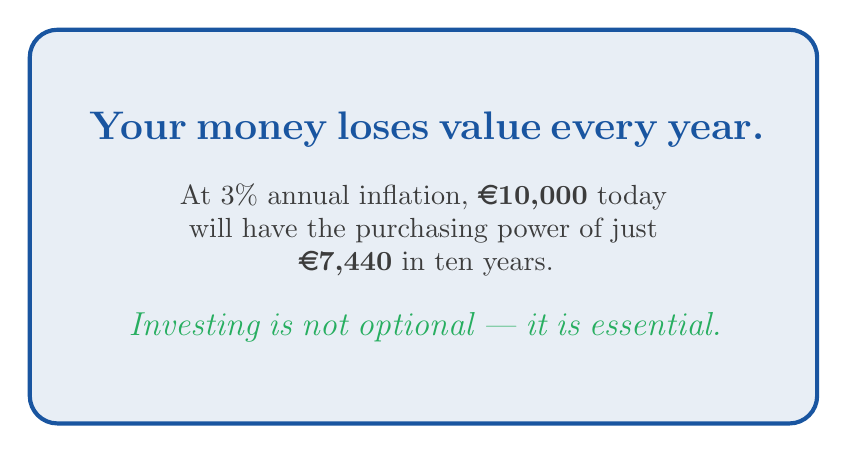
\begin{tikzpicture}
    \draw[fill=primaryblue!10, draw=primaryblue, line width=1.5pt, rounded corners=10pt]
      (0,0) rectangle (10,5);
    \node[align=center, text width=9cm] at (5,2.5) {
      \Large\color{primaryblue}
      \textbf{Your money loses value every year.}\\[0.4cm]
      \normalsize\color{darkgray}
      At 3\% annual inflation, \textbf{\euro{}10{,}000} today\\
      will have the purchasing power of just\\
      \textbf{\euro{}7{,}440} in ten years.\\[0.4cm]
      \large\color{secondarygreen}
      \textit{Investing is not optional --- it is essential.}
    };
  \end{tikzpicture}

  \vspace{2cm}

  {\large\color{darkgray} Targeted at adults aged \textbf{20--30}}\\[0.3cm]
  {\normalsize\color{darkgray} No prior financial knowledge required}

  \vfill

  {\color{primaryblue}\rule{\textwidth}{0.5pt}}\\[0.2cm]
  {\small\color{darkgray}
    \textit{This book is for educational purposes only and does not constitute financial advice.}\\
    \textit{Always consult a qualified financial advisor before making investment decisions.}
  }\\[0.3cm]
  {\small\color{darkgray} Financial Education Series \quad|\quad 2026 Edition}
\end{titlepage}

% ----------------------------------------------------------------
% TABLE OF CONTENTS
% ----------------------------------------------------------------
\tableofcontents
\thispagestyle{empty}

% ================================================================
\chapter*{Introduction: Why This Book Exists}
\addcontentsline{toc}{chapter}{Introduction: Why This Book Exists}
\markboth{Introduction}{}

You graduated, you got a job, you opened a bank account. You are told to ``save money'' --- so you do. Month after month, your salary arrives, you spend what you need, and you put the rest in your current account. Feels responsible, right?

Here is the uncomfortable truth: \textbf{saving money in a bank account is not the same as protecting your wealth.} In fact, with inflation running at 2--3\% per year (and historically higher), every euro sitting idle is silently losing value. After ten years at 3\% inflation, \euro{}10{,}000 buys roughly what \euro{}7{,}400 would buy today.

This book is written for people aged 20--30 who want to stop losing money passively and start building wealth actively --- without needing a finance degree, a wealthy family, or a crystal ball.

We will cover:
\begin{itemize}[leftmargin=1.5cm]
  \item Why inflation is your biggest long-term enemy
  \item How compound interest is your greatest long-term ally
  \item The three risk profiles: conservative, moderate, and aggressive
  \item Practical investment vehicles: ETFs, bonds, REITs, and more
  \item How to build a real portfolio based on who you are
  \item Common mistakes that destroy young investors
\end{itemize}

No jargon without explanation. No vague advice. Let's start.

% ================================================================
\chapter{Understanding Money, Inflation, and Time}

\section{What Is Inflation?}

Inflation is the rate at which the general level of prices for goods and services rises over time. When inflation is 3\%, a coffee that costs \euro{}1.00 today will cost \euro{}1.03 next year. This might seem trivial, but compounded over decades it becomes devastating for anyone who does not invest.

\begin{keybox}
\textbf{Purchasing Power} is how much a fixed amount of money can actually buy. As inflation rises, purchasing power falls. A \euro{}100 bill in 2006 could buy roughly what \euro{}138 buys in 2026 --- meaning its real value fell by 28\%.
\end{keybox}

The Eurozone has seen average inflation of around 2--3\% over the past two decades, with recent spikes above 8\% in 2022--2023. Even at the modest 2\% target of the European Central Bank, your money in a zero-interest account loses half its purchasing power in roughly 36 years.

\section{The Hidden Tax of Keeping Cash}

Most young people believe that ``not losing money'' means keeping it safe in a savings account. But consider the following comparison:

\begin{table}[h!]
\centering
\begin{tabular}{lccc}
\toprule
\textbf{Scenario} & \textbf{Start} & \textbf{After 10 years} & \textbf{After 20 years} \\
\midrule
Cash in account (0\% return) & \euro{}10{,}000 & \euro{}10{,}000 & \euro{}10{,}000 \\
Inflation at 3\% & \euro{}10{,}000 & \euro{}7{,}441 real value & \euro{}5{,}537 real value \\
Invested at 7\% avg. return & \euro{}10{,}000 & \euro{}19{,}672 & \euro{}38{,}697 \\
\bottomrule
\end{tabular}
\caption{The cost of inaction over 10 and 20 years (inflation-adjusted)}
\end{table}

The difference between the first and third row is not luck --- it is the decision to invest.

\section{Your Greatest Asset: Time}

When you are 25, you have something a 45-year-old investor would pay dearly for: \textbf{time}. Time is the engine behind compound interest, the most powerful force in personal finance.

\begin{examplebox}
\textbf{Compound Interest in Action:}\\[4pt]
\textbf{Alex} starts investing \euro{}200/month at age 25, earning an average 7\% annual return. By age 65, Alex has \textbf{\euro{}524{,}000}.\\[4pt]
\textbf{Jordan} waits until age 35 and invests the same \euro{}200/month at 7\%. By age 65, Jordan has only \textbf{\euro{}243{,}000}.\\[4pt]
The 10-year head start is worth \textbf{more than \euro{}280{,}000} --- without investing a single extra euro per month.
\end{examplebox}

\section{The Rule of 72}

The \textbf{Rule of 72} is a simple mental shortcut to estimate how long it takes for your money to double at a given annual return rate:

\[
\text{Years to double} = \frac{72}{\text{Annual Return (\%)}}
\]

\begin{table}[h!]
\centering
\begin{tabular}{cc}
\toprule
\textbf{Annual Return} & \textbf{Years to Double} \\
\midrule
2\% (high-yield savings) & 36 years \\
4\% (conservative portfolio) & 18 years \\
7\% (diversified equity fund) & ~10 years \\
10\% (aggressive growth) & ~7 years \\
\bottomrule
\end{tabular}
\caption{Rule of 72 applied to different return rates}
\end{table}

This simple rule illustrates why even a small increase in your average annual return has a profound impact over decades.

% ================================================================
\chapter{Before You Invest: Building Your Foundation}

\section{Step 1 --- Understand Where Your Money Goes}

Before putting a single euro into any investment, you need clarity on your cash flow. The classic \textbf{50/30/20 rule} offers a simple framework:

\begin{itemize}[leftmargin=1.5cm]
  \item \textbf{50\%} of take-home income $\rightarrow$ Needs (rent, food, transport, utilities)
  \item \textbf{30\%} of take-home income $\rightarrow$ Wants (dining out, entertainment, travel)
  \item \textbf{20\%} of take-home income $\rightarrow$ Savings \& Investments
\end{itemize}

If your income is tight, adapt this. Even 10\% invested consistently beats 20\% invested sporadically.

\section{Step 2 --- Kill High-Interest Debt First}

If you carry credit card debt at 15--20\% interest, investing elsewhere is almost always a losing trade. There is no stock or fund that reliably beats a guaranteed 20\% return --- which is exactly what paying off that debt gives you.

\begin{warningbox}
Pay off any debt with interest rates above 7--8\% before starting an investment portfolio. Student loans at 3--4\% can often be managed alongside investing. Credit cards cannot.
\end{warningbox}

\section{Step 3 --- Build an Emergency Fund}

An emergency fund is not an investment --- it is insurance. It protects you from being forced to sell investments at a loss when life happens: a medical bill, a car repair, unexpected unemployment.

Financial experts universally recommend:

\begin{itemize}[leftmargin=1.5cm]
  \item \textbf{Minimum:} 3 months of essential living expenses
  \item \textbf{Standard:} 6 months of living expenses
  \item \textbf{Extra security} (freelancer, irregular income): 9--12 months
\end{itemize}

Keep this money in a \textbf{high-yield savings account} or short-term money market fund --- accessible, but separated from your daily account to avoid temptation.

\begin{tipbox}
As of mid-2026, several online banks in Europe offer high-yield savings accounts paying 3--4\% annually with no lock-in period. This beats inflation at current rates while keeping liquidity.
\end{tipbox}

\section{Step 4 --- Define Your Goals}

Before choosing investments, ask yourself:
\begin{enumerate}[leftmargin=1.5cm]
  \item \textbf{What am I investing for?} (House deposit in 5 years? Retirement in 40 years? Financial freedom?)
  \item \textbf{When will I need this money?} (This determines how much risk you can afford)
  \item \textbf{How would I react if my portfolio dropped 30\%?} (This reveals your emotional risk tolerance)
\end{enumerate}

Honest answers to these three questions are the foundation of every good investment strategy.

% ================================================================
\chapter{Understanding Risk}

\section{What Is Investment Risk?}

In finance, \textbf{risk} is the possibility that your investment will deliver a return different from what you expected --- including a loss. Higher potential returns almost always come with higher risk. This is not a flaw in the system; it is how markets compensate investors for taking on uncertainty.

\begin{keybox}
\textbf{Risk and Return are inseparable.} A government bond might return 3\% with near-zero risk of loss. A single tech stock might return 30\% --- or drop 60\%. Understanding this trade-off is the core skill of investing.
\end{keybox}

\section{Two Types of Risk}

\begin{description}[leftmargin=1.5cm]
  \item[\textbf{Market Risk (Systematic)}] Affects the entire market --- recessions, geopolitical crises, pandemics. Cannot be eliminated by diversification.
  \item[\textbf{Specific Risk (Unsystematic)}] Affects a single company or sector --- a product failure, a CEO scandal, an industry disruption. \textit{Can} be reduced by holding a diversified portfolio.
\end{description}

\section{Your Risk Profile}

Your risk profile combines two things:
\begin{enumerate}[leftmargin=1.5cm]
  \item \textbf{Risk Capacity} --- How much loss can your financial situation actually absorb?
  \item \textbf{Risk Tolerance} --- How much volatility can you emotionally handle without panic-selling?
\end{enumerate}

Both matter equally. An investor who panic-sells every market dip earns far less than their portfolio's theoretical return.

\subsection{Factors That Affect Your Risk Profile}

\begin{table}[h!]
\centering
\begin{tabular}{lll}
\toprule
\textbf{Factor} & \textbf{Lower Risk Profile} & \textbf{Higher Risk Profile} \\
\midrule
Investment horizon & Short (< 5 years) & Long (10+ years) \\
Income stability & Freelance / variable & Salaried / stable \\
Existing savings & Low & High \\
Dependants & Many & None \\
Emotional reaction to loss & High anxiety & Calm, rational \\
Financial knowledge & Limited & Strong \\
\bottomrule
\end{tabular}
\caption{Factors influencing your risk profile}
\end{table}

In the next three chapters, we explore each risk profile in depth.

% ================================================================
\chapter{Risk Profile 1: The Conservative Investor}

\section{Who Is the Conservative Investor?}

You are a conservative investor if any of the following apply:
\begin{itemize}[leftmargin=1.5cm]
  \item You need your money within 1--5 years (e.g., saving for a house)
  \item A 20\% portfolio drop would cause you significant stress or force you to sell
  \item Your income is variable or you have limited savings outside of this investment
  \item You are completely new to investing and want to start small
\end{itemize}

Being conservative is not a weakness --- it is appropriate risk management for your situation.

\section{The Conservative Portfolio}

\begin{table}[h!]
\centering
\begin{tabular}{lcc}
\toprule
\textbf{Asset Class} & \textbf{Allocation} & \textbf{Expected Annual Return} \\
\midrule
Government Bonds (short/medium term) & 45\% & 3--4\% \\
Investment-Grade Corporate Bonds & 20\% & 4--5\% \\
Broad Market ETFs (equity) & 25\% & 6--8\% \\
Cash / High-Yield Savings & 10\% & 3--4\% \\
\midrule
\textbf{Portfolio Blended Return (est.)} & & \textbf{4--5\%} \\
\bottomrule
\end{tabular}
\caption{Conservative portfolio allocation}
\end{table}

\section{Investment Vehicles for Conservative Investors}

\textbf{Government Bonds (BTP, Bund, Treasury):} Loans you make to governments in exchange for fixed interest payments. Among the safest investments available, though they offer modest returns. Italian BTPs or German Bunds are common choices for European investors.

\textbf{Short-Duration Bond ETFs:} Instead of buying individual bonds, you buy an ETF that holds hundreds of bonds, providing instant diversification with low fees. Examples include \texttt{iShares EUR Govt Bond 1-3yr ETF} or \texttt{Xtrackers EUR Corporate Bond ETF}.

\textbf{Broad Market ETFs (small allocation):} Even conservative investors benefit from some equity exposure to beat inflation over time. A World ETF like \texttt{MSCI World} or \texttt{FTSE All-World} kept at 25\% provides growth without excessive volatility.

\begin{examplebox}
\textbf{Maria, 28 --- saving for a house in 4 years:}\\
Maria invests \euro{}400/month. She keeps \euro{}40 in high-yield savings, puts \euro{}180 in short-term bond ETFs, \euro{}80 in corporate bond ETFs, and \euro{}100 in a World ETF. Her expected annual return is \textasciitilde{}4.2\%. In 4 years, her \euro{}19{,}200 invested grows to approximately \textbf{\euro{}22{,}000} --- while staying protected from a severe market crash.
\end{examplebox}

\section{Key Risks to Watch}

\begin{warningbox}
Even ``safe'' bonds carry \textbf{inflation risk}: if your bond yields 3\% and inflation rises to 4\%, your real return is negative. For timescales over 5 years, a purely bond-based portfolio is not optimal.
\end{warningbox}

% ================================================================
\chapter{Risk Profile 2: The Moderate Investor}

\section{Who Is the Moderate Investor?}

You are a moderate investor if:
\begin{itemize}[leftmargin=1.5cm]
  \item Your investment horizon is 5--10+ years
  \item You could tolerate a 20--30\% portfolio drop without panic-selling --- but it would be uncomfortable
  \item You have a stable income and a solid emergency fund
  \item You want growth beyond inflation, but not the wild swings of an all-equity portfolio
\end{itemize}

Most people in their mid-20s to early 30s with stable employment fall into this category.

\section{The Moderate Portfolio}

\begin{table}[h!]
\centering
\begin{tabular}{lcc}
\toprule
\textbf{Asset Class} & \textbf{Allocation} & \textbf{Expected Annual Return} \\
\midrule
Broad Equity ETFs (global) & 55\% & 7--9\% \\
Bond ETFs (mix of govt + corporate) & 30\% & 3--5\% \\
REITs (Real Estate Investment Trusts) & 10\% & 5--7\% \\
Cash / Liquidity Buffer & 5\% & 3\% \\
\midrule
\textbf{Portfolio Blended Return (est.)} & & \textbf{6--7\%} \\
\bottomrule
\end{tabular}
\caption{Moderate portfolio allocation}
\end{table}

\section{Investment Vehicles for Moderate Investors}

\textbf{Global Equity ETFs:} The workhorse of the moderate portfolio. ETFs like \texttt{Vanguard FTSE All-World (VWCE)} or \texttt{iShares MSCI World (IWDA)} give you exposure to thousands of companies across 50+ countries in a single, low-cost fund. Average expense ratios: 0.07--0.22\% per year.

\textbf{Bond ETFs:} A 30\% bond allocation cushions the portfolio during equity market downturns. In 2022, when global stocks fell \textasciitilde{}18\%, high-quality bond ETFs acted as a stabilizer for balanced portfolios.

\textbf{REITs (Real Estate Investment Trusts):} REITs are companies that own income-producing real estate (offices, malls, warehouses, apartments). By law, they must distribute at least 90\% of taxable income to shareholders as dividends. They provide:
\begin{itemize}[leftmargin=1.5cm]
  \item Real estate exposure without needing large capital
  \item Regular dividend income (typically 3--6\% yield)
  \item Low correlation to traditional stocks and bonds
\end{itemize}

\texttt{iShares Developed Markets Property Yield ETF} (IWDP) is a widely-used option for European investors.

\section{The Power of Dollar-Cost Averaging (DCA)}

For moderate investors investing monthly from salary, Dollar-Cost Averaging is the ideal strategy:

\begin{keybox}
\textbf{Dollar-Cost Averaging (DCA)} means investing a \textit{fixed amount} at \textit{regular intervals} (e.g., \euro{}300 every first day of the month), regardless of market conditions.\\[4pt]
When prices are high, you buy fewer units. When prices are low, you buy more. Over time, this reduces the average cost per unit and removes the temptation to ``time the market.''
\end{keybox}

Research consistently shows that for investors without the ability to perfectly time the market (i.e., everyone), DCA reduces emotional decision-making, lowers average purchase costs during volatile periods, and builds the discipline necessary for long-term wealth accumulation.

\begin{examplebox}
\textbf{Luca, 26 --- building long-term wealth:}\\
Luca earns \euro{}2{,}000/month net. He invests \euro{}300/month: \euro{}165 into a MSCI World ETF, \euro{}90 into a bond ETF, \euro{}30 into a REIT ETF, and keeps \euro{}15 in a liquidity buffer. At a blended 6.5\% return over 20 years, his total investment of \euro{}72{,}000 grows to approximately \textbf{\euro{}138{,}000}.
\end{examplebox}

\section{Rebalancing: Staying on Target}

Over time, a strong equity rally will push your stock allocation above target. \textbf{Rebalancing} means selling some of the outperformer and buying the underperformer to restore your target weights. Do this once or twice a year, not constantly.

% ================================================================
\chapter{Risk Profile 3: The Aggressive Investor}

\section{Who Is the Aggressive Investor?}

You are an aggressive investor if:
\begin{itemize}[leftmargin=1.5cm]
  \item You have a 10+ year horizon and will not need this money soon
  \item You could see your portfolio drop 40--50\% and stay calm --- understanding it is temporary
  \item You have a stable income, no high-interest debt, and a solid emergency fund
  \item You want to maximize long-term wealth, and are willing to accept short-term volatility as the price
\end{itemize}

This profile is \textit{particularly} well-suited to people in their 20s --- because time is the greatest buffer against market volatility.

\section{The Aggressive Portfolio}

\begin{table}[h!]
\centering
\begin{tabular}{lcc}
\toprule
\textbf{Asset Class} & \textbf{Allocation} & \textbf{Expected Annual Return} \\
\midrule
Global Equity ETFs (broad market) & 60\% & 7--9\% \\
Sector / Thematic ETFs & 20\% & 8--12\% \\
Emerging Markets ETFs & 10\% & 8--11\% \\
Crypto (Bitcoin / Ethereum only) & 5\% & High volatility \\
REITs & 5\% & 5--7\% \\
\midrule
\textbf{Portfolio Blended Return (est.)} & & \textbf{8--10\%} \\
\bottomrule
\end{tabular}
\caption{Aggressive portfolio allocation}
\end{table}

\section{Investment Vehicles for Aggressive Investors}

\textbf{Broad Equity ETFs (core):} The foundation remains a globally diversified ETF. The core 60\% follows the same logic as the moderate portfolio --- but at a higher weight, without the bond ballast.

\textbf{Thematic / Sector ETFs (satellite):} These are ETFs focused on specific high-growth sectors:
\begin{itemize}[leftmargin=1.5cm]
  \item Technology: \texttt{iShares S\&P 500 IT Sector ETF}
  \item Clean Energy: \texttt{iShares Global Clean Energy ETF}
  \item Healthcare / Biotech: \texttt{iShares MSCI World Health Care ETF}
\end{itemize}
These carry more risk but offer higher growth potential. Limit thematic bets to the satellite portion of your portfolio.

\textbf{Emerging Markets ETFs:} Countries like India, Brazil, Vietnam, and Indonesia offer faster GDP growth than developed markets. Emerging market ETFs (e.g., \texttt{iShares MSCI Emerging Markets ETF}) capture this growth --- with higher volatility. A 10\% allocation adds return potential without overexposure.

\textbf{Cryptocurrency (5\% cap):} Crypto is highly speculative. Bitcoin (BTC) and Ethereum (ETH) are the only two assets with a sufficient track record for inclusion in a portfolio. Morgan Stanley and most institutional advisors cap crypto at 2--10\% of total assets. Important rules:
\begin{itemize}[leftmargin=1.5cm]
  \item \textbf{Never invest more than you can afford to lose completely}
  \item Expect drawdowns of 30--60\% --- they are normal in crypto
  \item Long-term holders (``HODLers'') statistically outperform active traders
  \item Do not use leverage or derivatives
\end{itemize}

\begin{warningbox}
Crypto is not a ``get rich quick'' tool. It is a high-risk, high-reward speculative asset. Many young investors have lost significant sums by overexposing themselves or trading on emotions. A 5\% cap is not timidity --- it is risk management.
\end{warningbox}

\begin{examplebox}
\textbf{Sofia, 23 --- maximising long-term growth:}\\
Sofia invests \euro{}250/month aggressively from her first job. After 30 years at an average 8.5\% annual return, her total contribution of \euro{}90{,}000 becomes approximately \textbf{\euro{}380{,}000}. If she had kept that money in cash losing 2\% real value per year, she would have roughly \euro{}49{,}000 in real purchasing power.
\end{examplebox}

% ================================================================
\chapter{The Investment Toolkit}

\section{Stocks (Equities)}

A stock represents partial ownership of a company. When the company grows, your share grows in value. When it pays dividends, you receive a portion of its profits.

\textbf{Pros:} High long-term return potential, liquidity, dividend income.\\
\textbf{Cons:} Individual stocks carry high specific risk; requires research and monitoring.

\textbf{Verdict for young investors:} Do not build a portfolio of individual stocks as a beginner. Use ETFs to get broad equity exposure with far less risk.

\section{ETFs (Exchange-Traded Funds)}

An ETF is a basket of assets (stocks, bonds, or other) that trades on an exchange like a single stock. It provides:
\begin{itemize}[leftmargin=1.5cm]
  \item \textbf{Instant diversification} across hundreds or thousands of assets
  \item \textbf{Low fees} --- quality ETFs have expense ratios as low as 0.03\%
  \item \textbf{Transparency} --- you always know what is inside
  \item \textbf{Liquidity} --- buy or sell any time the market is open
\end{itemize}

For most young investors, a \textbf{two-fund or three-fund portfolio} built from ETFs is all that is needed:
\begin{enumerate}[leftmargin=1.5cm]
  \item A global equity ETF (e.g., \texttt{VWCE} --- Vanguard FTSE All-World)
  \item A bond ETF (e.g., \texttt{AGGH} --- iShares Core Global Aggregate Bond)
  \item Optionally: a REIT ETF (e.g., \texttt{IWDP})
\end{enumerate}

\section{Bonds}

A bond is a loan you make to a government or company in exchange for fixed interest payments (the ``coupon'') and return of principal at maturity.

\begin{table}[h!]
\centering
\begin{tabular}{lll}
\toprule
\textbf{Bond Type} & \textbf{Risk Level} & \textbf{Typical Yield} \\
\midrule
Government (e.g., German Bund) & Very Low & 2--3\% \\
Investment-Grade Corporate & Low--Medium & 3--5\% \\
High-Yield (``Junk'') Corporate & Medium--High & 6--9\% \\
TIPS / Inflation-Linked & Low & Inflation + 1\% \\
\bottomrule
\end{tabular}
\caption{Bond types and their risk/return characteristics}
\end{table}

\textbf{TIPS (Treasury Inflation-Protected Securities)} and their European equivalents (OATi, BTPei) are especially relevant: their principal adjusts with inflation, making them a direct hedge against rising prices.

\section{REITs (Real Estate Investment Trusts)}

REITs allow anyone to invest in real estate without buying property. They are publicly traded companies owning real estate portfolios, and they must pay out at least 90\% of their income as dividends. They provide real asset exposure, income, and inflation protection (rents tend to rise with inflation).

\section{Index Funds vs. Active Funds}

\begin{keybox}
Decades of data show that \textbf{over 80\% of actively managed funds underperform their benchmark index} over a 10-year period --- and the gap widens after fees. For most investors, low-cost index funds are superior to active management.
\end{keybox}

The average active fund charges 1--1.5\% annually. On a \euro{}100{,}000 portfolio over 20 years, the difference between a 0.2\% ETF and a 1.2\% active fund is approximately \textbf{\euro{}25{,}000} in extra fees alone.

% ================================================================
\chapter{Building Your Portfolio: Step by Step}

\section{Step 1 --- Choose a Broker}

To invest, you need a brokerage account. Key criteria for young European investors:

\begin{itemize}[leftmargin=1.5cm]
  \item \textbf{Low fees:} Look for zero-commission platforms or very low flat-rate fees
  \item \textbf{ETF availability:} Ensure access to a wide range of ETFs (especially UCITS-compliant for EU investors)
  \item \textbf{Regulation:} Always use a broker regulated by ESMA, FCA, or equivalent national authority
  \item \textbf{Tax reporting:} Some brokers provide annual tax reports, simplifying your tax return
\end{itemize}

Popular platforms in Europe include DEGIRO, Scalable Capital, Trade Republic, and Fineco (in Italy). Always check current fees before opening an account.

\section{Step 2 --- Select Your Profile and Allocation}

Use the framework from chapters 4--6 to identify your profile. Then select your target allocation. Write it down. Print it. This is your \textbf{Investment Policy Statement} --- a personal commitment to your strategy.

\section{Step 3 --- Automate and Forget}

Set up a monthly automatic transfer from your current account to your investment account. Then set up automatic purchase orders for your ETFs.

\begin{tipbox}
Automation is the single most powerful behavioral tool available to investors. It removes emotion, ensures consistency, and prevents you from spending money before it gets invested. Treat your monthly investment like a fixed bill --- not an optional extra.
\end{tipbox}

\section{Step 4 --- Review, Not React}

Check your portfolio \textbf{once a quarter at most}. Do not open your broker app during market crashes --- your only action should be to keep investing as scheduled (or even increase your purchases, since assets are on sale).

Annual rebalancing: once per year, review whether your actual allocation drifted significantly from your target, and adjust.

% ================================================================
\chapter{Common Mistakes to Avoid}

\section{Trying to Time the Market}

``I'll invest when the market corrects.'' This is the most common error. Markets spend far more time going up than down. Missing the 10 best trading days in any given 20-year period can cut your total return by \textbf{more than half}. The correct answer to ``when should I invest?'' is almost always: \textit{now, and every month after that}.

\section{Panic Selling During Crashes}

Every significant market crash in history --- 2000, 2008, 2020 --- was followed by a full recovery and new highs. Investors who sold during the 2020 COVID crash locked in losses; those who held (or bought more) saw their portfolios recover within months.

\begin{keybox}
Market downturns are not the end of your portfolio --- they are a \textbf{sale on future returns}. For a young investor in the accumulation phase, falling prices are an opportunity, not a disaster.
\end{keybox}

\section{Overconcentrating in a Single Asset}

Whether it is your employer's stock, your country's market, or a hot cryptocurrency, over-concentration is how ordinary investors suffer catastrophic losses. Diversification is the only free lunch in investing.

\section{Ignoring Fees}

1\% per year sounds trivial. Over 30 years on a \euro{}100{,}000 portfolio growing at 7\%, the difference between a 0.2\% fee and a 1.2\% fee is approximately \euro{}100{,}000 in lost wealth. Fees are the most controllable variable in your investment returns.

\section{Waiting for the ``Perfect'' Moment}

Analysis paralysis kills more investment returns than bad market timing. An imperfect portfolio started today beats a perfect strategy that never gets started. Start small if needed --- \euro{}50/month is enough to build habits and experience while your income grows.

\section{Confusing Speculation with Investing}

Day trading, leveraged products, complex derivatives, meme stocks, and most crypto ``opportunities'' are speculation, not investing. Speculation can make you rich quickly --- and lose everything just as fast. Investing is boring, slow, and extraordinarily effective over time.

% ================================================================
\chapter{Bringing It All Together}

\section{A Summary by Risk Profile}

\begin{table}[h!]
\centering
\renewcommand{\arraystretch}{1.4}
\begin{tabular}{>{\bfseries}p{2.5cm}p{2.5cm}p{2.5cm}p{2.5cm}}
\toprule
 & \textbf{Conservative} & \textbf{Moderate} & \textbf{Aggressive} \\
\midrule
Horizon & 1--5 years & 5--10 years & 10+ years \\
Bonds & 65\% & 30\% & 0\% \\
Equities & 25\% & 55\% & 85\% \\
REITs & 0\% & 10\% & 5\% \\
Crypto & 0\% & 0\% & 5\% \\
Cash & 10\% & 5\% & 5\% \\
Est. Return & 4--5\% & 6--7\% & 8--10\% \\
Max Drawdown & \textasciitilde{}10--15\% & \textasciitilde{}25--30\% & \textasciitilde{}40--50\% \\
\bottomrule
\end{tabular}
\caption{Summary comparison of the three risk profiles}
\end{table}

\section{Your First 90 Days --- An Action Plan}

\begin{enumerate}[leftmargin=1.5cm]
  \item[\textbf{Week 1--2:}] Calculate your monthly income, expenses, and how much you can invest. Identify and begin paying off high-interest debt.
  \item[\textbf{Week 3--4:}] Open a high-yield savings account and start building your emergency fund. Target 3 months of expenses within 6--12 months.
  \item[\textbf{Month 2:}] Research regulated brokers available in your country. Open an account. Spend time learning the platform on paper before investing real money.
  \item[\textbf{Month 3:}] Make your first investment. Start small if necessary. Set up automated monthly contributions. Choose your ETFs based on your risk profile.
  \item[\textbf{Ongoing:}] Invest every month. Check quarterly. Rebalance annually. Increase contributions as your income grows. Never stop.
\end{enumerate}

\section{The Mindset That Makes It Work}

Portfolio selection matters less than \textbf{behavior}. The investors who build wealth are not the ones with the cleverest strategies --- they are the ones who invest consistently through market cycles, ignore media panic, and let time do the work.

Your 20s are not too early to start investing. They are exactly the right time. Every month you wait is a month of compound growth you cannot get back.

\begin{tipbox}
Start now. Start small. Stay the course.\\[4pt]
These six words have built more wealth than any advanced financial theory ever invented.
\end{tipbox}

% ================================================================
\chapter*{Glossary of Key Terms}
\addcontentsline{toc}{chapter}{Glossary of Key Terms}
\markboth{Glossary}{}

\begin{description}[leftmargin=2cm, style=nextline]
  \item[\textbf{Asset Class}] A category of investment with similar characteristics: equities, bonds, real estate, cash.
  \item[\textbf{Bond}] A fixed-income instrument where the investor lends money to a borrower (government or company) and receives regular interest payments plus principal at maturity.
  \item[\textbf{Compound Interest}] Earning returns on both your original investment and the returns already accumulated. The core mechanism of long-term wealth building.
  \item[\textbf{Diversification}] Spreading investments across different asset classes, sectors, and geographies to reduce overall portfolio risk.
  \item[\textbf{Dollar-Cost Averaging (DCA)}] Investing a fixed amount at regular intervals regardless of market conditions.
  \item[\textbf{ETF (Exchange-Traded Fund)}] A fund that tracks an index or basket of assets and trades on a stock exchange like a share.
  \item[\textbf{Expense Ratio}] The annual fee charged by a fund, expressed as a percentage of assets.
  \item[\textbf{Inflation}] The rate at which the general price level rises, eroding the purchasing power of money.
  \item[\textbf{Liquidity}] How quickly and easily an asset can be converted to cash without significantly affecting its price.
  \item[\textbf{Portfolio}] The complete collection of investments owned by an individual or institution.
  \item[\textbf{REIT}] Real Estate Investment Trust --- a company owning income-producing real estate that must distribute 90\%+ of income to shareholders.
  \item[\textbf{Risk Tolerance}] The degree of variability in investment returns an investor is willing to withstand.
  \item[\textbf{TIPS}] Treasury Inflation-Protected Securities --- government bonds whose principal adjusts with inflation.
  \item[\textbf{Volatility}] The degree to which an asset's price fluctuates over time. High volatility = higher uncertainty.
\end{description}

% ================================================================
\chapter*{Disclaimer}
\addcontentsline{toc}{chapter}{Disclaimer}
\markboth{Disclaimer}{}

This book is intended for educational and informational purposes only. Nothing in this book constitutes personalised financial, tax, or investment advice. All investments involve risk, including the possible loss of principal. Past performance of any asset class or strategy does not guarantee future results.

Before making any investment decisions, readers are strongly encouraged to consult with a qualified, regulated financial adviser who can assess their individual circumstances, financial situation, and goals.

The figures, return estimates, and portfolio examples used in this book are illustrative only and are based on historical averages. Actual results will vary. The names and examples in this book are fictional and used for illustrative purposes only.

\vspace{1cm}
{\small\textit{``An investment in knowledge pays the best interest.''} --- Benjamin Franklin}

% ================================================================
\end{document}
